\documentclass[12pt,titlepage]{article}

% \usepackages21{fancyhdr}

\usepackage[printwatermark]{xwatermark}

\usepackage{grffile}
\usepackage{xcolor}
\usepackage{lipsum}
\usepackage{times}
\usepackage{soul}
\usepackage{epsfig}
\usepackage{rotating}
\usepackage{url}
\usepackage{latexsym}
\usepackage{graphicx}
\usepackage{amsfonts}
\usepackage{amsmath, amsthm, amssymb}
\usepackage{fullpage}
\usepackage{setspace}
\usepackage{natbib}
\usepackage{longtable}
\usepackage{keyval}
\usepackage{caption,subcaption}
\usepackage{arydshln}
%%\usepackage[hyphenbreaks]{breakurl}

%% allow urls to get broken on hyphens
\usepackage{hyperref}
\def\UrlBreaks{\do\/\do-}


%% APSR submission: no commas in citations between name and year
%% See http://merkel.zoneo.net/Latex/natbib.php
\bibpunct{(}{)}{;}{author-year}{}{;}

% the opening bracket symbol, default = (
% the closing bracket symbol, default = )
% the punctuation between multiple citations, default = ;
% the letter `n' for numerical style, or `s' for numerical superscript style, any other letter for author-year, default = author-year;
% the punctuation that comes between the author names and the year
% the punctuation that comes between years or numbers when common author lists are suppressed (default = ,);

\usepackage{footmisc}
\renewcommand{\footnotelayout}{\doublespacing} % set spacing in footnotes
\newlength{\myfootnotesep}
\setlength{\myfootnotesep}{\baselineskip}
\addtolength{\myfootnotesep}{-\footnotesep}
\setlength{\footnotesep}{\myfootnotesep} % set spacing between footnotes

% make footnote font size same as regular font size in text
\renewcommand{\footnotesize}{\normalsize} 


%% Use this for a "DRAFT" watermark
%% \newwatermark[allpages,color=pink!50,angle=45,scale=5,xpos=-25,ypos=40]{DRAFT}

%% List all locations for graphics here
\graphicspath{ {../plots/} }


\begin{document}
\sloppy
\thispagestyle{empty}

%% APSR submission requires double-spaced footnotes
%%\newcommand{\footnote}[1]{\footnote{\doublespacing #1}} %% <-- note \doublespacing here.

\renewcommand{\topfraction}{.85}
\renewcommand{\bottomfraction}{.7}
\renewcommand{\textfraction}{.15}
\renewcommand{\floatpagefraction}{.66}
\renewcommand{\dbltopfraction}{.66}
\renewcommand{\dblfloatpagefraction}{.66}

\newcommand{\yi}{\ensuremath{Y_i}}

% \urldef\myurlncsl1\url{foo%.com}
% \begin{document}
% text\footnote{WWW: \myurl}


\title{\Large{All in the family:\\Anna and Lisa Hahner's finishing
    times in\\the 2016 women's Olympic
  marathon}}\author{David Cottrell\thanks{Postdoctoral Research
  Fellow, Program in Quantitative Social Science, Dartmouth College,
    6108 Silsby Hall, Hanover, NH
    03755 (\texttt{david.cottrell@dartmouth.edu}).} \and Michael C.\
  Herron\thanks{Visiting Scholar, Hertie School of Governance, Berlin,
    Germany, and Professor of Government, Dartmouth College, 6108
    Silsby Hall, Hanover, NH 03755
    (\texttt{michael.c.herron@dartmouth.edu}).}}


\maketitle \doublespacing 

%\begin{abstract} 
% \noindent
%The abstract
%\end{abstract}

%\newpage


\begin{quote}
  \emph{``I invested all I had and 300 meters before the finish line,
    I was next to Lisa. It was a magical moment that we could finish
    this marathon together. We did not think about what we were
    doing.'' -- Anna Hahner}
\end{quote}


\section*{Introduction}

On August 14, 2016, at 9:30 in the morning, the Women's Olympic
marathon kicked off in Rio de Janeiro, Brazil, when 156 runners from
80 countries across the world left the starting line en route to their
destination 42.195 kilometers away. Two hours, twenty-four minutes,
and four seconds later, Jemima Sumgong of Kenya would be the first to
cross the finishline and take home gold; Sumgong was just 3.5 minutes
behind her personal best time in the marathon. Approximately 21
minutes later, twin marathoners from Germany, Anna and Lisa Hahner,
would cross the finishline together, holding hands and celebrating a
personal victory. Although the Hahners would finish 81st and 82nd,
respectively, with times slightly more than 18 minutes slower than
corresponding personal bests, Anna Hahner would describe their joint
finish as a ``magical moment.''
\href{https://www.nytimes.com/2016/08/17/sports/olympics/twins-finish-marathon-hand-in-hand-but-their-country-says-they-crossed-a-line.html}
The media quickly picked up on the Hanher story as an image of the
beaming twins finishing hand-in-hand captured a public audience. Many
believed the moment was a reflection of the Olympic spirit.

Not everyone agreed with this rosy interpretation. The twins' happy
facial expressions at the finish were portrayed as a bit contrived
(smiling like ``Honigkuchenpferde''---a Honigkuchenpferd is a German
cookie in the shape of a horse), and the sports director of the German
Athletics Federation, Thomas Kurschilgen, stirred up controversy when
he suggested that the Hahners' photo-finish was no coincidence.
Kurschilgen averred that the twins slowed down so as to finish
simultaneously and create a spectacle which would ``generate media
attention.'' Kurschilgen justified his charge with the fact that the
twins ran in the Rio marathon at least 18 minutes slower their
personal best times prior to the
Olympics.\footnote{\url{https://www.nytimes.com/2016/08/17/sports/olympics/twins-finish-marathon-hand-in-hand-but-their-country-says-they-crossed-a-line.html}}
Not surprisingly, these accusations were denied by the Hahner twins,
who claimed that their simultaneous finish was simply an unintended
coincidence.

%% Honigkuchenpferd quote from here:
%%
%% https://www.welt.de/sport/olympia/article157669264/Das-falsche-Laecheln-der-deutschen-Lauf-Zwillinge.html


What happened in the women's Olympic marathon, and how might we
develop a statistical approach that assesses whether the Hahner finish
was coincidental or intentional?  These two interpretations are
clearly at odds. If the former, then the Hahner twins are to be
celebrated and their finish treated as an expression of the spirit
behind the Olympic games. If the latter, though, then the twins may
have violated this spirt by not trying hard enough. It is perhaps too
easy for us to write such a glib sentence---neither of us cannot
fathom being able to complete a marathon anywhere in the vicinity of
two and a half hours---but we nonetheless want to know what the data
from the Olympic marathon data tell us.  Was the Hahner finish in the
2016 women's Olympic marathon a lovely coincidence or something else?

Among female Olympic marathoners, the Hahner twins were not alone in
their familial ties, and we draw on this in the analysis that follows.
The marathon also featured twins from North Korea, Kim Hye-song and
Kim Hye-gyong, who posted identical times and finished 10th and 11th
in the race, respectively. The Kim finish, unlike the Hahner finish,
appears devoid of post-race controversy. Moreover, three triplets from
Estonia competed in the Rio marathon, although only two, Lily Luik and
Leila Luik, finished it, in 97th and 114th place, respectively. The
third Estonia triplet, Liina Luik, recorded what is known as a
DNF---an abbreviation that means did not finish, a term that we will
use throughout this article.

\section*{Marathon data and our research design}

For each participant who started the women's Olympic marathon, we know
several things: personal best marathon time prior to the 2016 Olympic
games; split times from the Rio marathon course at 5 kilometers, 10
kilometers, and so forth; and, finishing time. We cannot directly
observe the effort that an individual put into the race, and we do not
know why some runners have DNF results.  Some runners may have injured
themselves on the course and accordingly dropped out, and others may
have dropped out, uninjured, in anticipation of an unsatisfactory
result. Of the 156 marathon starters, 133 completed the race and 23
DNFed at various locations throughout the course. The overall DNF rate
was thus $\frac{23}{156} \approx 0.15$, and the relatively small
sample size at our disposal means that a 95\% confidence for this rate
is fairly wide, namely, $\left(0.098, 0.22\right)$.  Key in the
analysis that follows is the deviation between a runner's Rio time and
her prior personal best time in the marathon.  While there is variance
across runners in these deviations, they nonetheless may be able to
provide us with insight as to the Hahner twins' performance in the
marathon.

Our research design has two components.  In the first, we present some
visualizations that present the Hahner twin's results in context; our
interest here is primarily the two Hanhers although we comment on the
Kim twins and Luik triplets when appropriate.  Our visualizations
suggest blah blah bhah.  We then turn to a modeling approach and in
particular a simulation.  In simulated Olympic marathons, which we
develop based on relationships (excluding twins and triplets) between
known personal best times and observed Rio finishing times, we find
that the Hahner twins finished suspiciously close to each other given
the disparty between their personal best times.  OR THEY DID NOT.

\section*{Visualizing the Olympic marathon}

SOME PLOTS HERE.  Maybe PB versus FINAL and HALF vs Final.  

As a brief overview of the race, Figure \ref{fig:secondsbehind}
describes each runner's status at the various split times on the
marathon course.  Each dot in the figure depicts a recorded split and
the number of seconds each runner was behind the race leader at the
time.  There are more dots at earlier splits due to the accumulation
of DNFs.  Regarding twins and triplets, the Estonian Luik triplets are
denoted with blue dots; there are three blue dots through the 20
kilometer split, but the third triplet did not record a half-marathon
split.  The orange dots in the figure represent the Hahner twins; as
noted in the figure, Lisa Hahner was ahead of her sister through 15
kilometers at which point Anna surged ahead.  Lastly, Figure
\ref{fig:secondsbehind} contains two red dots representing the North
Korean Kim twins; this is not visually apparent because the Kim twins
had identical split times during the marathon.

\begin{figure}[!ht]
  \centering
  \caption{Runner status by split}
  \label{fig:secondsbehind}
  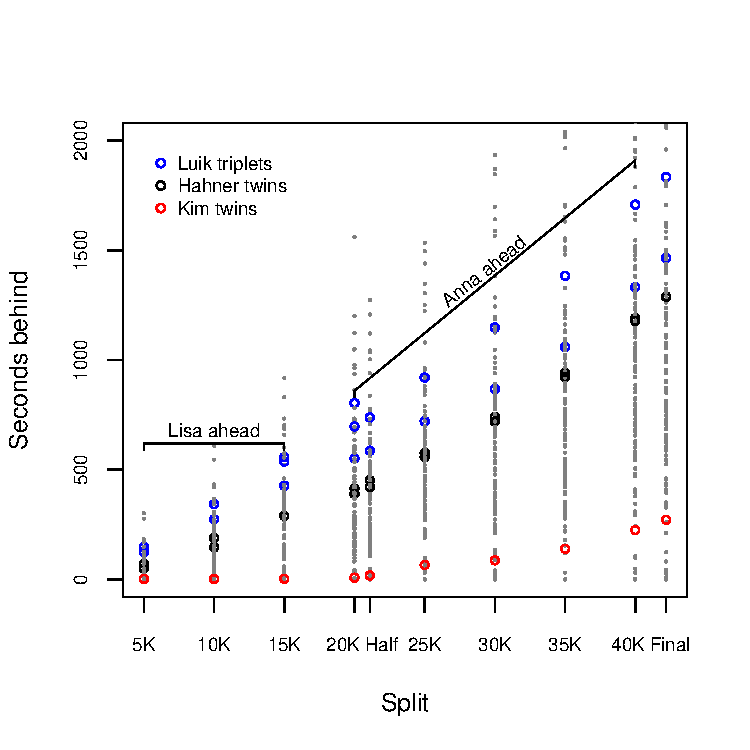
\includegraphics[scale = 1]{seconds-behind.pdf}
  \begin{flushleft}
    \emph{Note: each dot represents one runner at a split.  DNFs are
      not pictured, and splits are not to scale.}
  \end{flushleft}
\end{figure}

Figure \ref{fig:secondsbehind} does not directly shed any light on our
motivating research question, but it does show that the Hahner twins
finished amidst many other runners.  We will come back to this point
later.

\section*{The probability of an unintentional simultaneous finish}

Thomas Kurschilgen's accusations of an intentional finish stems from
two observations. First, the Hahner twins finished slower than he
expected given respective personal bests. Second, the twins finished
together at the exactly same time. Kurschilgen clearly believed that
neither of these events would have occurred had both Hahner run the
marathon independently, absent coordination. By his logic, the German
twins should have run faster and not have finished simultaneously.

On the other hand, only a handful of runners completed the Rio
marathon with times that were faster than their recorded best times.
Thus, 18 minutes behind a personal record may not be the outlier that
Kurschilgen claimed it to be. Moreover, there is good reason to
suspect that an unintended simultaneous finish was more likely for the
Hahner twin than it would be for any other set of runners. After all,
these two women are twins with presumably similar abilities. Not only
do they train together, but their pre-Rio best times are less than two
minutes apart. While Anna may be slightly faster than Lisa measured by
personal bests, we might expect the difference in their Rio result to
be just as close as the differences in their recorded bests. And given
random variation in finishing times, a simultaneous finish might not
be out of the ordinary.

Even though they seem similar, finishing at very similar times and
finishing together are different phenomena. If, for example, both
Hahners were of similar ability to each other and also to many other
runners, then we might expect similar finishing times yet not
necessarily similar placements. The latter will be a function of the
extent to which all runners on the Rio course have similar talent
levels.  This point is an important one and will be evident in the
results that follow.

To test the assertion that the Hahner twins paced themselves to finish
at the same time and with back-to-back placements, we need to compute
the probability that such a result would have occurred
unintentionally. Hence we need to know the probability distribution of
Anna and Lisa's finishing times if their runs had been independent of
each other. The challenge, of course, is that this distribution is
unknown.  % Therefore it needs to be estimated.

\section*{Modeling}

%% THIS SECTION IS A MESS.  I JUST WANTED TO PUT SOMETHING IN WRITING.

%% Ok!  Not sure what all the notation means.

% We know that Anna and Lisa Hahner finished the marathon in Rio
% simultaneously. We don't know, however, if the finish was intentional;

The Hahner twins either acted independently $I$ or coordinated their
times $C$; these are the two possible states of the race
$\psi = \{I, C\}$. Given that we observed Anna and Lisa's finishing
times, $Y_A = y_A$ and $Y_L = y_L$, we want to know the probability
that they ran independently, as they say they did. Hence, we are
looking to determine, %% y_a versus Y_a.  Former realized?

$$P(\psi = I \mid y_A  \cap y_L )$$

However, to determine this, we need to have some understanding of a
likelihood function that specifies Rio finishing times. We want to
know the likelihood of Anna's and Lisa's final times given
independence $P(y_A \cap y_L \mid \psi = I )$. We can estimate this
function with a few assumptions. First, we assume that under
independence, any given runner's final time $Y_i$ is conditional on
his/her running ability plus noise. Specifically, we assume that the
$Y_i$ is a linear function of the runner's ability $X_i$ plus a
normally distributed error term $e_i \sim N(0, \sigma)$. Second, we
assume that every runner shares the same linear relationship - meaning
the slope and intercept remain constant across runners. Third, we
assume that the error term is drawn from a common distribution across
runners. Hence, luck and misfortune are drawn from the same
distribution. Therefore,

$$Y_i \sim N(\beta_0 + X_{i}\beta_1 + e_i, \sigma)$$

We also assume that a runner's ability $X_i$ can be measured precisely
by her best marathon performance leading up to the Olympics. 

%% Any measurement error must therefore be negligible.

If Anna and Lisa intentionally slowed down as a result of coordination
then we would likely observe $y_A > E(Y_A \mid \psi = I) $ and
$y_L > E(Y_L\mid \psi = I )$. In other words, the final times that
Anna and Lisa recorded in the race would be greater than we would
expect if they had run independently.

Moreover, if Anna and Lisa coordinated to finish simultaneously, then
the difference between the two sisters' final times would be less that
the expected difference had they run independently. Therefore, under a
coordinated finish we would expect
$\left|y_A - y_L\right| < E(\left|Y_A - Y_L\right| \mid \psi = I )$.

\section*{Did Anna and Lisa intentionally slow down?}

According to Kurschilgen, Anna and Lisa underperformed in the Rio marathon. He claimed that because their goal was to finish simultaneously rather than finish at their fastest pace, their times were slower than they otherwise would have been.  He claimed that the twins were simply trading speed for a photo-finish.

If this were the case, the function generating Anna and Lisa's final times would deviate from the function that generated everyone else's final times.  Given everyone else would draw their times from the independent distribution  $Y_i \sim N(\beta_0 + X_{i}\beta_1 + e, \sigma)$,  Anna and Lisa would draw from a distribution of times that are slower in expectation. Hence, they would lie well-above the line that links a runner's performance in Rio to their previous best performance.    

\begin{figure}[!ht]
  \caption{Relationship between Personal Best and Result  -- caption?}
  \label{fig:scatter}
  \begin{subfigure}{.5\textwidth}
    \centering
    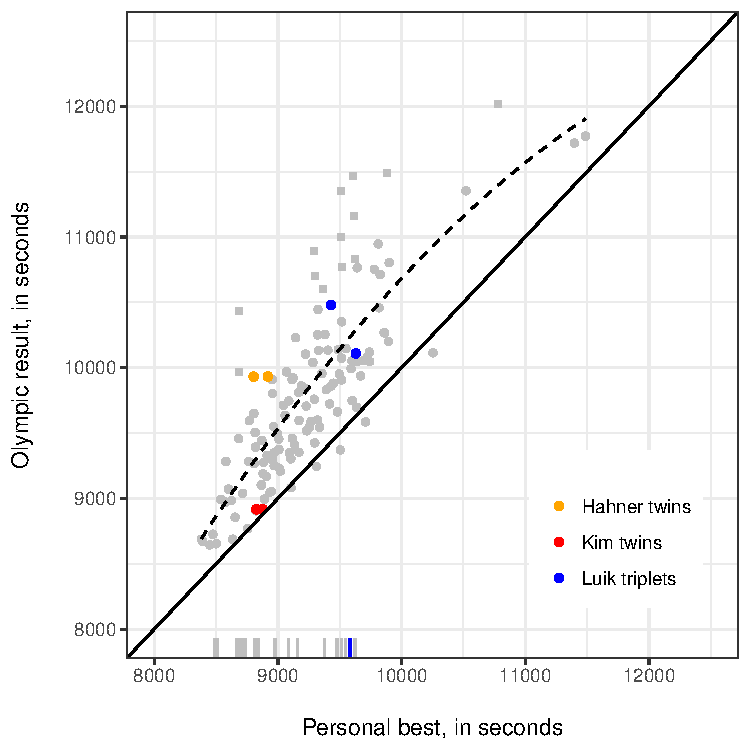
\includegraphics[width=\textwidth,
    keepaspectratio]{scatter_plot.pdf}
    \caption{Rio finishing times and personal best times}
    \label{fig:45degreeplot}
  \end{subfigure}
  \begin{subfigure}{.5\textwidth}
    \centering
    % \label{fig:Studentized Residuals}
    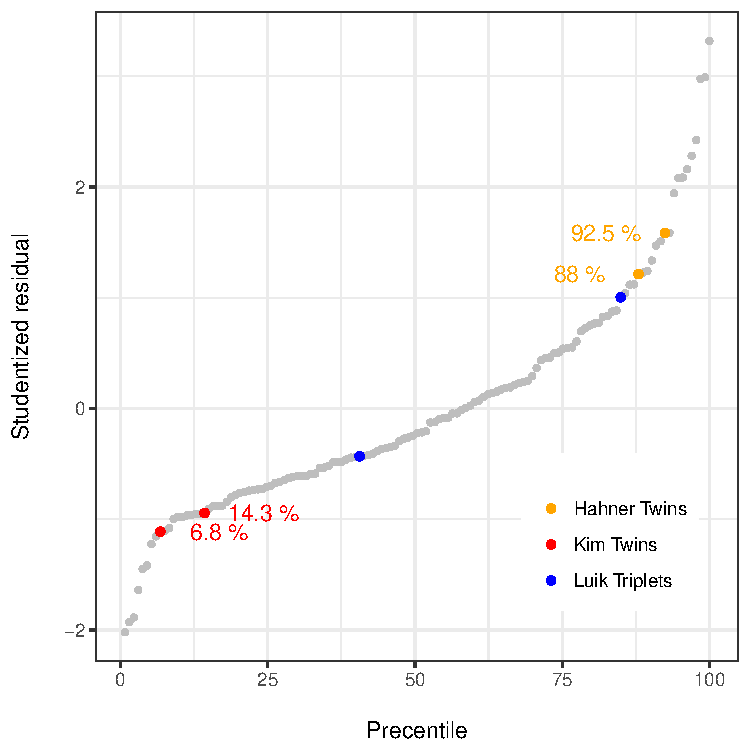
\includegraphics[width=.975\textwidth, keepaspectratio]{studentized_residuals.pdf}
    \caption{Studentized residuals}
    \label{fig:studentizedresiduals}
  \end{subfigure}
\end{figure}

Figure \ref{fig:45degreeplot} displays the relationship between a
runner's personal best (horizontal axis) and her final result
(vertical axis).  The 133 finishers are plotted as grey points, and
the 23 DNFs are depicted below along the horizontal axis with
tick-marks.  The dashed black line with grey confidence intervals
represent ordinarily least squares estimates of the linear
relationship between racer's finishing and personal best times.

One can see in Figure \ref{fig:scatter} that there is a clear
relationship between a runner's personal best time and her performance
in the Olympics.  While there is a significant amount of noise in the
relationship, the Hahner twins' dots are well above the regression's
fitted line notwithstanding this point.  They finished the Rio
marathon much slower than they should have, per their pre-Olympic
personal best times.  In fact, if we sort studentized residual, we can
see in Figure \ref{fig:studentizedresiduals} that the Hahner twins are
in the tail-end of the residual distribution.  Anna Hahner's residual
deviation is greater than 91.7\% of the runners who completed the
marathon while Lisa Hahner's deviation is greater than 86.5\%.  Hence,
the twins appear to have finished at a much slower pace than expected,
which is what we might expect if they were coordinating their runs.
The North Korean Kim twins are also in the tail of the residual
distribution---but the left tail.  These twins finished much faster
than expected. 

\section*{Did Anna and Lisa intentionally finish together?}

Anna and Lisa finished the marathon at an unusually slow rate, which is what we might expect if the twins intentionally slowed their pace to finish simultaneously.  However, the observation of a slow finish does not necessarily imply that it was an intentional result .  It only suggests that Kurschilgen's claim regarding this issue holds up in the data.

Perhaps it would be easier to refute the claim if we could show that the Twins's back-to-back finish was not such an unusual event.  Given that Anna and Lisa were so close in their personal best times, it may seem reasonable to expect that they would also be close in their finishing times.   Hence, one way to determine if the twins's finish was intentional is to quantify the likelihood that such a close finish would occur by chance given the differences in their ability. 

We can attempt to quantify this likelihood by looking at how differences in the personal best time of two runners translate into differences in Olympic times .  If Anna and Lisa's finish was unintentional we'd expect that such a close finish would be unlikely given their difference in personal best times.   Yet, how does the difference in personal best times relate to the difference in finishing times?

One way we can estimate this relationship is to look at all of the differences that we observe in the marathon.  We can take the difference in personal best time for every combination of runners in the data and look at the difference in their final times.  We should expect that compared to the difference in their personal best times, the difference in Anna and Lisa's final times should be commensurate with the conditional difference of all other runners. %This needs a better explanation.

Therefore, we find all combinations of runners in the marathon and calculate two quantities: 1) the difference in their personal best time and 2) the difference in their final time. We plot the relationship between the two quantities in Figure \ref{fig:diffdiffscatter}.   All 8,778 dyadic combinations of runners are displayed by grey points in the scatter plot.   The solid black line indicates a one-to-one relationship, where every point would fall if the difference in final times were systematically equivalent to the difference in personal bests.  


\begin{figure}[!ht]
 \caption{Relationship between Difference in Personal Best and Difference in Result}
 \label{fig:diffdiffscatter}
 \centering
 \begin{subfigure}{.5\textwidth}
 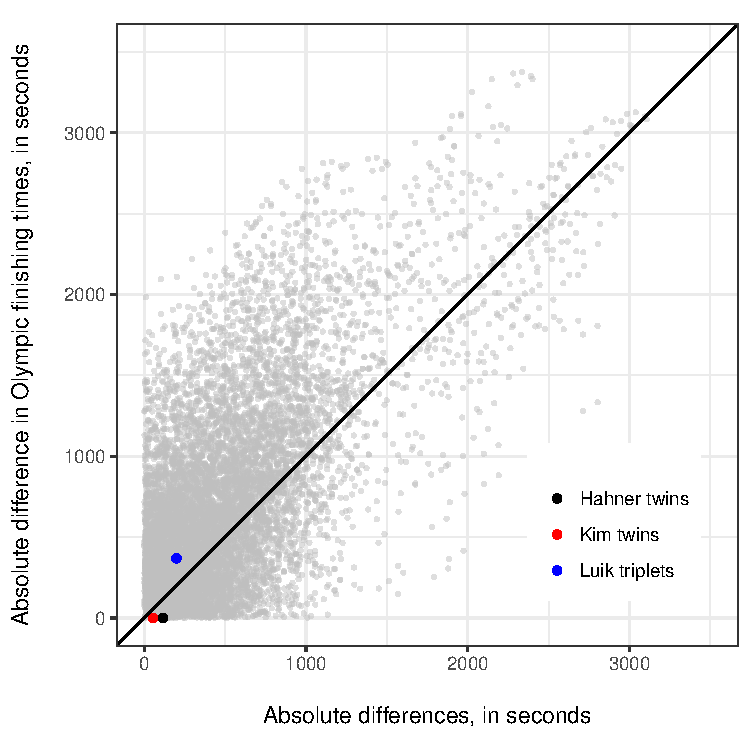
\includegraphics[width=\textwidth, keepaspectratio]{diff_in_diff_scatter_plot.pdf}
 \end{subfigure}
\end{figure}

We can see from the yellow dot that the Hahner Twins are just below this one-to-one line.  Hence, the twins' final times were closer to each other than their personal best times; but not by much.  In fact, this might be an expected difference if we expected there to be a one-to-one relationship.     However, although there is a clear relationship between the difference in final time and the difference in personal best, it is not a strong one-to-one relationship.  We've added a dotted smoother to display a cubic splines estimate of the conditional averages.  While the Hahner twins may be close to the one-to-one line, they are much further away from the average set of runners.  Hence, we would expect for any pair of runners, the difference in their final results should be much greater than their difference in their personal best.  However, the Hahner twins do not fit this expectation.   Yet, how different from this expectation are they?

One way we can quantify the degree to which the twins are outliers is by comparing their difference in difference to every other pair of runner's difference-in-differences.  We calculate the difference-in-differences for each pair of runners by simply subtracting their difference in result (y-axis) from their difference in personal best (x-axis).  Therefore positive difference-in-differences mean that the runners ended up further apart than their difference in personal bests.  Negative difference-in-differences mean that the runners end up closer together.  Hence, the Hahner twins have a difference-in-difference of -114 seconds.  They finished 114 seconds closer together than the distance between their personal bests.  

We arrange all 8,778 difference-in-differences from small to large in the first plot in Figure \ref{fig:diffdiff}. The Hahner twins are denoted by the yellow point.  Using this plot we can visualize where the twins fall within the distribution of difference-in-differences.  It is clear that they are closer to the lower tail of the distribution.  However, compared to all other difference-in-differences, their result is not that extreme.  Nearly 21\% of the difference-in-dfferences were less than the that of the twins'. Hence, we'd expect at least one in five pairs of runners to have a reduction in difference at least as great as the twins.

However, if we limit the observations to only those runners who had personal best times that were at least as close to each other as the Hahner twins, we get a different persepective.  Among those runners,  the Hahner twins reduced the distance between them to the greatest extent.  There was no other pair of runners whose reduced the difference in the final time relative to their difference in personal bests more than them.         

\begin{figure}[!ht]
 \caption{How Hahner Twins Rank in Difference-in-Differences}
 \label{fig:diffdiff}
 \begin{subfigure}{.5\textwidth}
 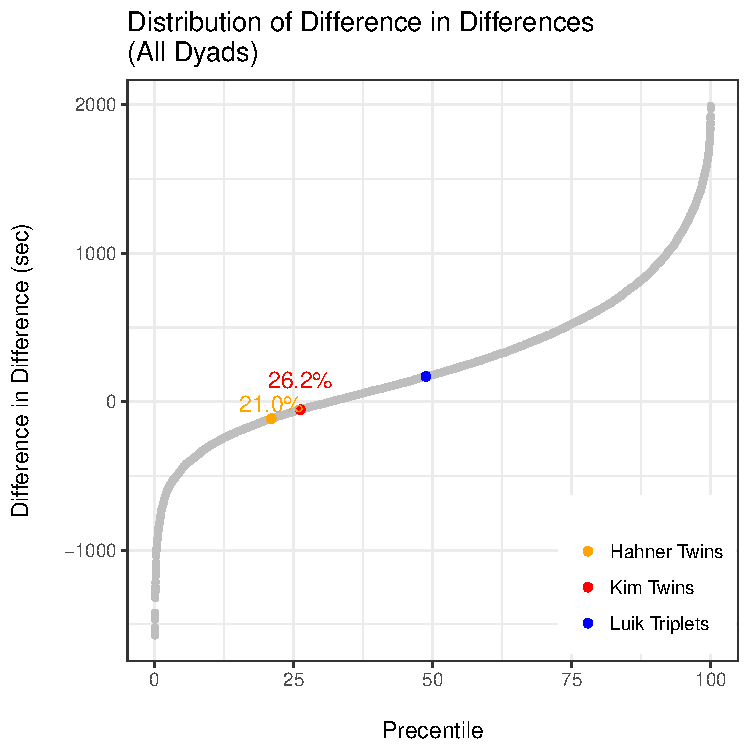
\includegraphics[width=\textwidth, keepaspectratio]{diff_in_diff_1.pdf}
 \end{subfigure}
 \begin{subfigure}{.5\textwidth}
 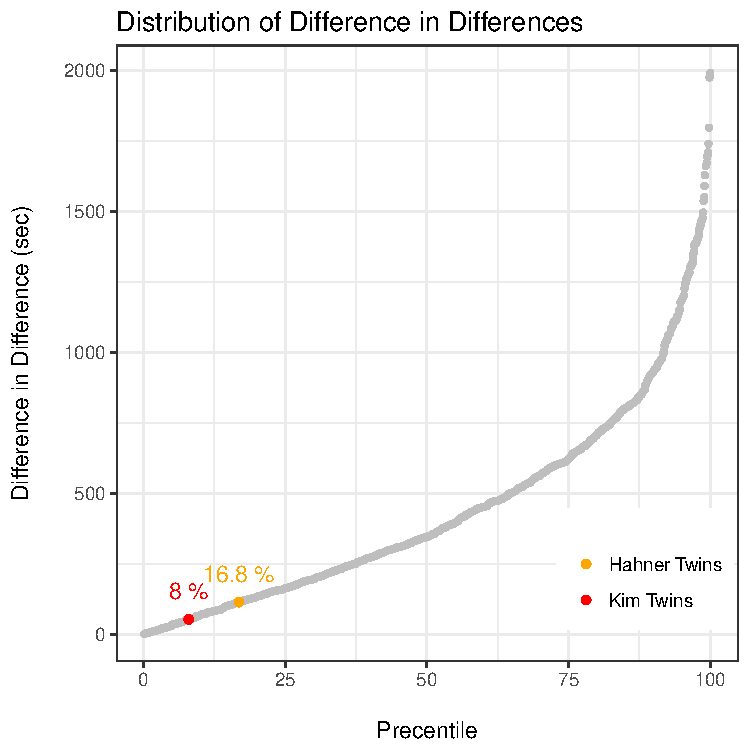
\includegraphics[width=\textwidth, keepaspectratio]{diff_in_diff_2.pdf}
 \end{subfigure}
\end{figure}

\newpage
\subsection*{Steps of the simulation}

\begin{enumerate}
\item Removing the two sets of twins and triplets from the sample,
  estimate a linear model that predicts a runner's final time ($Y_i$)
  based on her pre-Olympic personal best time ($X_i$).
\item Extract the coefficients and the variance-covariance matrix from
  this model.
\item For each runner, draw $\beta_0$ and $\beta_1$ from a multivariate normal
distribution with mean equal to the coefficients and variance equal to the
variance-covariance matrix.
\item For each runner, draw an error term ($e$) from a normal distribution with
mean equal to zero and a standard deviation equal to the standard
deviation of the model's residuals ($\sigma$).
\item For each runner, predict the final result by combining the randomly
  generated beta coefficients and error terms, $\hat{y} = \beta_0 + \beta_1 + e$.
\item Eliminate each runner from the race with a probability equal to the
percent of the total runners who did not finish in the actual race.  This
account for the likelihood of a DNF.
\item Calculate the difference in time between Anna Hahner and Lisa Hahner.
\item Calculate the difference in ranking between Anna Hahner and Lisa Hahner.
\item Repeat steps 3 through 8 ten thousand times.
\item Plot a histogram of the results in Figure \ref{fig:simdiff}
\end{enumerate}

\begin{figure}[!ht]
  \centering
  \caption{Distribution of simulated results for the Hahner twins}
  \label{fig:simdiff}
  \begin{subfigure}{.45\textwidth}
    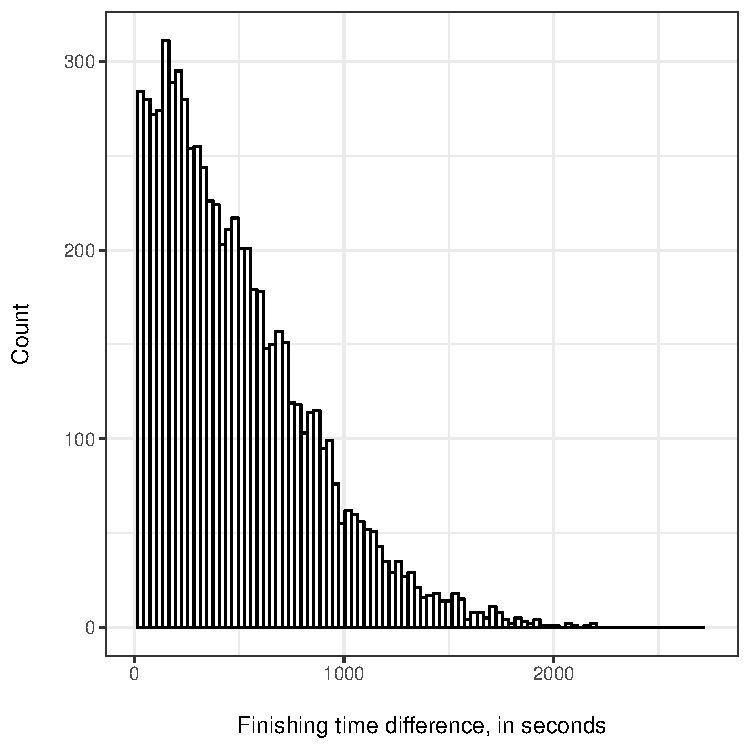
\includegraphics[width=\textwidth,
    keepaspectratio]{simulated_time.pdf}
    \caption{Simulated differences in finishing times}
    \label{fig:simulatedfinishtimes}
  \end{subfigure}
  \begin{subfigure}{.45\textwidth}
    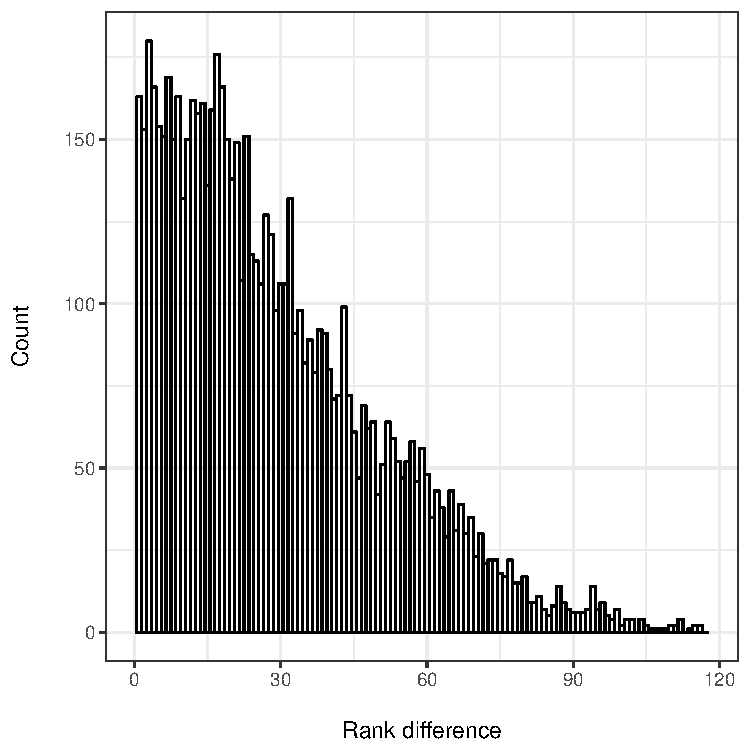
\includegraphics[width=\textwidth, keepaspectratio]{simulated_rank.pdf}
    \caption{Simulated differences in places}
    \label{fig:simulatedranks}
  \end{subfigure}
\end{figure}






   

\end{document}

